\section{Startseite}
\label{home}

Wird die Webseite zum Ersten mal aufgerufen, wird die Startseite (Home-view) angezeigt. 

\begin{figure}[H]
    \begin{center}
      \frame{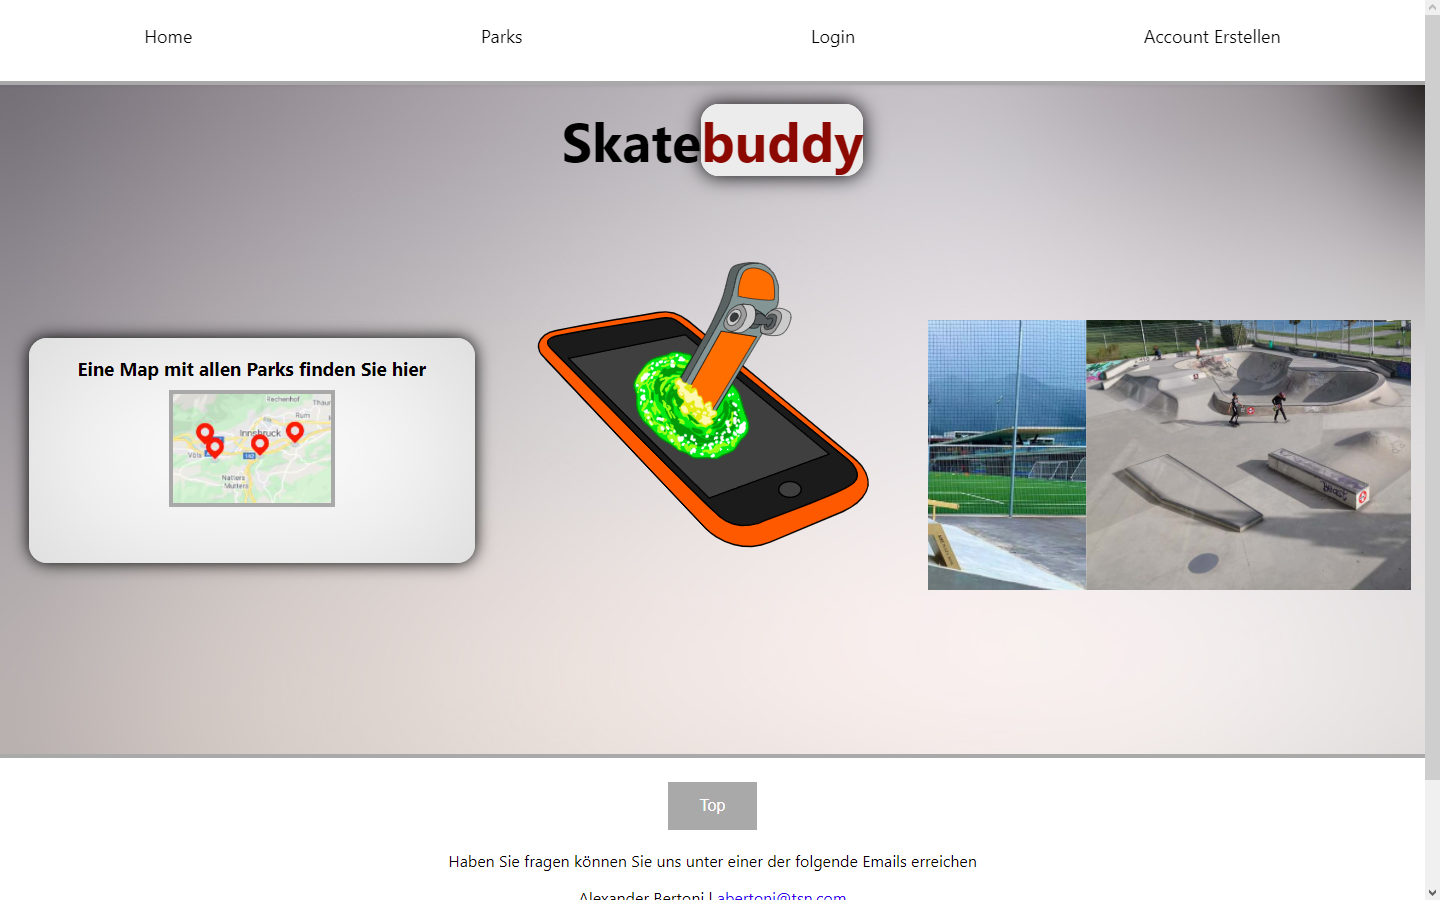
\includegraphics[width=0.8\textwidth]{Website/Home-page.png}}
      \caption{Die Startseite}
    \end{center}
\end{figure}

Hier befindet sich das \underline{\nameref{logo}} des Projekts, als sowohl auch ein Knopf welcher zu einer \underline{\nameref{map}} mit Überblick über alle 
Parks weiterleitet. Rechts vom Logo befindet sich eine \underline{\nameref{slideshow}} welche immer zwischen die ersten Bilder 
aller Parks umschaltet. Drückt der Benutzer auf die Slideshow gelangt dieser auf die \underline{\nameref{parkDetails}}
Seite des Parks, dem das Bild gehört. 
